\documentclass[12pt,a4paper]{article}
\usepackage{amsmath, amssymb, geometry, booktabs, xcolor, hyperref,
            listings, pgfplots, tcolorbox, enumitem, fancyhdr, tikz, array}
\geometry{margin=2.5cm}
\pgfplotsset{compat=1.18}
\tcbuselibrary{skins, breakable}

% ── tcolorbox environments ────────────────────────────────────────────────────
\newtcolorbox{curiositybox}[1]{colback=yellow!10, colframe=orange!80!black,
  fonttitle=\bfseries, title=#1, breakable}
\newtcolorbox{infobox}[1]{colback=blue!5, colframe=blue!60!black,
  fonttitle=\bfseries, title=#1, breakable}
\newtcolorbox{mistakebox}[1]{colback=red!5, colframe=red!60!black,
  fonttitle=\bfseries, title=#1, breakable}
\newtcolorbox{learnbox}[1]{colback=green!5, colframe=green!60!black,
  fonttitle=\bfseries, title=#1, breakable}

% ── lstlisting for Python ─────────────────────────────────────────────────────
\lstset{language=Python, basicstyle=\ttfamily\small, keywordstyle=\color{blue},
        commentstyle=\color{gray}, stringstyle=\color{orange},
        showstringspaces=false, numbers=left, numberstyle=\tiny,
        breaklines=true, frame=single}

% ── fancyhdr ──────────────────────────────────────────────────────────────────
\pagestyle{fancy}
\fancyhf{}
\lhead{Topic 07: Special Functions}
\rhead{Unit IV --- Laplace Transforms}
\cfoot{\thepage}

% ── title ─────────────────────────────────────────────────────────────────────
\title{Topic 07: Special Functions \\ \large Unit IV --- Laplace Transforms}
\author{23A54201 --- Mathematics IV (Transform Techniques) \\
        JNTUA College of Engineering (Autonomous)}
\date{}

% ─────────────────────────────────────────────────────────────────────────────
\begin{document}
\maketitle
\tableofcontents
\newpage

% ═════════════════════════════════════════════════════════════════════════════
%  OPENING HOOK
% ═════════════════════════════════════════════════════════════════════════════
\begin{curiositybox}{Hook}
A light switch turns on at $t = 2$ seconds. An explosion happens instantaneously
at $t = 3$ seconds. A filter processes a signal with a fractional power decay
$t^{-1/2}$. None of these can be described using elementary functions
alone --- you need special functions. The unit step function captures the switch,
the Dirac delta captures the explosion, and the Gamma function captures the
fractional power. Each has a Laplace transform. This topic gives you all three,
plus two more.
\end{curiositybox}

% ═════════════════════════════════════════════════════════════════════════════
\section{Why This Topic Exists}
% ═════════════════════════════════════════════════════════════════════════════

Before we begin, here is the honest answer to why you are reading this\ldots

Real engineering signals include sudden switches, impulse forces, and fractional
powers --- none of which are handled by the elementary functions covered in
Topics 04--06. If you try to model a circuit that switches on at $t = 2\,s$ with
a sine or exponential, you will obtain the wrong differential equation. The
special functions in this topic were invented precisely to fill these gaps.

\medskip
\begin{center}
\begin{tabular}{>{\bfseries}p{6cm} p{8cm}}
\toprule
Mistake & Consequence \\
\midrule
Not knowing the unit step function &
  Unable to represent piecewise inputs compactly; forced into case-by-case
  analysis that breaks when solving ODEs systematically. \\
\midrule
Treating $\delta(t)$ as an ordinary function with a finite value &
  Mathematical errors in impulse response calculations; integrals of $\delta$
  give wrong answers. \\
\midrule
Ignoring the Gamma function &
  Cannot compute $\mathcal{L}\{t^n\}$ for non-integer $n$; entire class of
  filter and signal problems becomes inaccessible. \\
\bottomrule
\end{tabular}
\end{center}

\begin{learnbox}{Key Takeaway}
Every special function in this topic was invented to solve a real problem.
Treat each one as a tool with a specific job, and your toolkit becomes
significantly more powerful.
\end{learnbox}

% ═════════════════════════════════════════════════════════════════════════════
\section{You Already Know This (Intuition First)}
% ═════════════════════════════════════════════════════════════════════════════

Think of a craftsman's toolbox. When you first learn woodworking you buy a
hammer, a screwdriver, and a saw --- the elementary tools. These handle the
vast majority of jobs. But the moment you need to tighten a bicycle wheel you
reach for a torque wrench; when wiring a circuit you grab wire strippers. These
are \emph{specialised} tools, invented because a specific job kept coming up
and none of the general tools handled it cleanly.

Special functions work the same way. The elementary functions --- powers,
exponentials, sines --- are the hammer and screwdriver. The unit step function,
Dirac delta, Gamma function, error function, and Bessel functions are the
specialised tools. Each was invented or formalised because a specific class of
engineering problem appeared repeatedly and the basic toolkit fell short.

By the end of this topic you will have five new tools in your transform toolkit,
each with a clear Laplace transform and a clear use-case.

% ═════════════════════════════════════════════════════════════════════════════
\section{The Unit Step Function (Heaviside Function)}
% ═════════════════════════════════════════════════════════════════════════════

\begin{infobox}{Definition and Laplace Transform of $u(t-a)$}

\textbf{Definition.} The \emph{unit step function} (or Heaviside function) is
\[
  u(t - a) = \begin{cases} 0 & t < a \\ 1 & t \geq a \end{cases}
\]
also written $H(t-a)$. The special case $a = 0$ gives $u(t) = u(t-0)$, which is
$1$ for all $t \geq 0$ and $0$ for $t < 0$.

\medskip
\textbf{Laplace Transform --- Derivation.}
\begin{align*}
  \mathcal{L}\{u(t-a)\}
  &= \int_0^{\infty} e^{-st}\, u(t-a)\, dt \\
  &= \int_a^{\infty} e^{-st}\, dt
     \quad \text{(since } u(t-a) = 0 \text{ for } t < a\text{)} \\
  &= \left[ \frac{e^{-st}}{-s} \right]_a^{\infty} \\
  &= 0 - \frac{e^{-as}}{-s} \\[4pt]
  &= \boxed{\dfrac{e^{-as}}{s}}, \quad s > 0.
\end{align*}

\medskip
\textbf{Writing Piecewise Functions Using Unit Steps.}
Any piecewise function
\[
  f(t) = \begin{cases} g_1(t) & 0 \leq t < a \\ g_2(t) & t \geq a \end{cases}
\]
can be written as
\[
  f(t) = g_1(t) + \bigl[g_2(t) - g_1(t)\bigr]\, u(t-a).
\]
This converts a case-by-case definition into a single algebraic expression that
can be transformed term-by-term using the Second Shifting Theorem:
\[
  \mathcal{L}\{g(t-a)\,u(t-a)\} = e^{-as}\,G(s), \quad G(s) =
  \mathcal{L}\{g(t)\}.
\]

\end{infobox}

\subsection{Worked Example: Piecewise Function via Unit Steps}

\begin{infobox}{Example --- Writing a Piecewise Function and Finding Its Transform}

\textbf{Problem.} Let
\[
  f(t) = \begin{cases} 3t & 0 \leq t < 4 \\ 12 & t \geq 4 \end{cases}.
\]
Express $f(t)$ using unit step functions and hence find $\mathcal{L}\{f(t)\}$.

\medskip
\textbf{Step 1 --- Rewrite using unit steps.}

Here $g_1(t) = 3t$ and $g_2(t) = 12$.
\[
  f(t) = 3t + (12 - 3t)\,u(t-4).
\]
Note that $12 - 3t = -3(t - 4) + 0$, so we write $12 - 3t = -3(t-4)$
evaluated at general $t$. We need to express $(12 - 3t)$ in terms of $(t-4)$
for the shifting theorem:
\[
  12 - 3t = -3(t - 4).
\]
Hence
\[
  f(t) = 3t - 3(t-4)\,u(t-4).
\]

\textbf{Step 2 --- Apply the Laplace transform.}
\begin{align*}
  \mathcal{L}\{f(t)\}
  &= \mathcal{L}\{3t\} - 3\,\mathcal{L}\{(t-4)\,u(t-4)\} \\
  &= 3 \cdot \frac{1}{s^2} - 3\,e^{-4s} \cdot \frac{1}{s^2}
     \quad \text{(Second Shifting Theorem with } g(t) = t\text{)} \\
  &= \frac{3}{s^2} - \frac{3e^{-4s}}{s^2} \\[4pt]
  &= \boxed{\dfrac{3(1 - e^{-4s})}{s^2}}.
\end{align*}

\end{infobox}

\begin{learnbox}{What Did We Learn?}
To use the Second Shifting Theorem, rewrite every piece of the piecewise
function so that each factor alongside $u(t-a)$ is expressed as a function
of $(t-a)$, not bare $t$. Then $\mathcal{L}\{g(t-a)\,u(t-a)\} = e^{-as}G(s)$
applies directly.
\end{learnbox}

\subsection{Graphs of the Unit Step Function}

\begin{center}
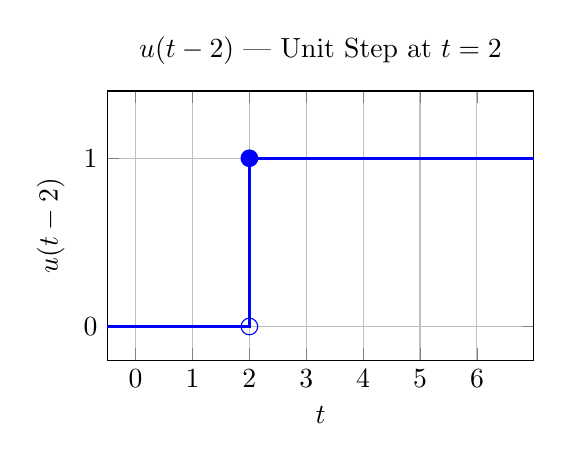
\begin{tikzpicture}
\begin{axis}[
  title={$u(t-2)$ --- Unit Step at $t=2$},
  xlabel={$t$}, ylabel={$u(t-2)$},
  xmin=-0.5, xmax=7, ymin=-0.2, ymax=1.4,
  grid=major,
  width=7cm, height=5cm,
  xtick={0,1,2,3,4,5,6},
  ytick={0,1}
]
  \addplot[blue, very thick, const plot] coordinates {(-0.5,0)(2,1)(7,1)};
  \addplot[blue, mark=o, mark size=3pt, only marks] coordinates {(2,0)};
  \addplot[blue, mark=*, mark size=3pt, only marks] coordinates {(2,1)};
\end{axis}
\end{tikzpicture}
\hspace{1cm}
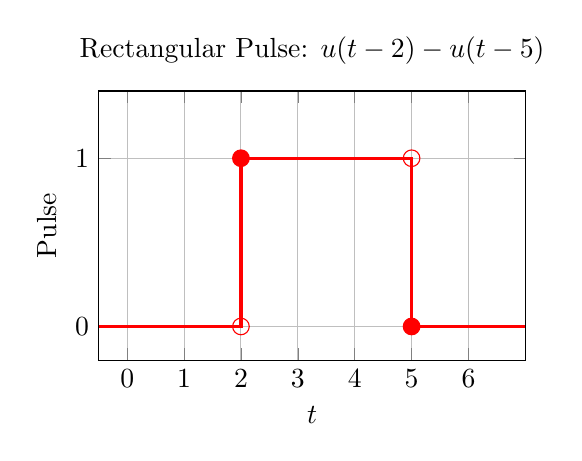
\begin{tikzpicture}
\begin{axis}[
  title={Rectangular Pulse: $u(t-2) - u(t-5)$},
  xlabel={$t$}, ylabel={Pulse},
  xmin=-0.5, xmax=7, ymin=-0.2, ymax=1.4,
  grid=major,
  width=7cm, height=5cm,
  xtick={0,1,2,3,4,5,6},
  ytick={0,1}
]
  \addplot[red, very thick, const plot]
    coordinates {(-0.5,0)(2,1)(5,0)(7,0)};
  \addplot[red, mark=o, mark size=3pt, only marks] coordinates {(2,0)(5,1)};
  \addplot[red, mark=*, mark size=3pt, only marks] coordinates {(2,1)(5,0)};
\end{axis}
\end{tikzpicture}
\end{center}

\begin{learnbox}{Reading the Graphs}
$u(t-2)$ stays zero until $t=2$, then jumps to 1 and stays there. The
rectangular pulse $u(t-2)-u(t-5)$ is 1 only on the interval $[2,5)$ and zero
everywhere else --- the standard way to ``window'' a signal.
\end{learnbox}

% ═════════════════════════════════════════════════════════════════════════════
\section{The Dirac Delta Function (Impulse Function)}
% ═════════════════════════════════════════════════════════════════════════════

\begin{infobox}{Definition and Laplace Transform of $\delta(t-a)$}

\textbf{Motivation.} Think of a hammer blow on a structure. The force is
enormous but lasts only an instant. Mathematically, model it as the limit of a
rectangular pulse of height $1/\varepsilon$ and width $\varepsilon$ as
$\varepsilon \to 0$. The area (impulse) is always 1.

\medskip
\textbf{Defining properties:}
\[
  \delta(t - a) = 0 \quad \text{for } t \neq a, \qquad
  \int_{-\infty}^{\infty} \delta(t - a)\, dt = 1.
\]

\medskip
\textbf{Sifting property.} For any function $f$ continuous at $t = a$:
\[
  \int_{-\infty}^{\infty} f(t)\,\delta(t - a)\, dt = f(a).
\]
This is the defining operational property of $\delta(t-a)$.

\medskip
\textbf{Laplace Transform --- Derivation using the sifting property.}
\begin{align*}
  \mathcal{L}\{\delta(t-a)\}
  &= \int_0^{\infty} e^{-st}\,\delta(t-a)\, dt \\
  &= e^{-sa} \quad \text{(sifting property with } f(t) = e^{-st},\ a \geq 0\text{)} \\[4pt]
  &= \boxed{e^{-as}}, \quad a \geq 0.
\end{align*}
Special case $a = 0$: $\mathcal{L}\{\delta(t)\} = 1$.

\medskip
\textbf{Engineering applications:}
\begin{itemize}
  \item \textbf{Impulsive mechanical force:} a hammer blow at time $a$
        modelled as $F_0\,\delta(t-a)$.
  \item \textbf{Instantaneous charge injection:} in a circuit, injecting
        charge $Q$ at $t = a$ gives a current $I(t) = Q\,\delta(t-a)$.
  \item \textbf{Initial condition modelling:} a system at rest but with a
        non-zero initial velocity can be modelled using $\delta(t)$ forcing.
\end{itemize}

\end{infobox}

\subsection{Schematic Diagram of the Dirac Delta}

\begin{center}
\begin{tikzpicture}
  \draw[->] (-0.5,0) -- (5,0) node[right] {$t$};
  \draw[->] (0,-0.3) -- (0,3.2) node[above] {Amplitude};
  \draw[blue, very thick, ->] (2.5,0) -- (2.5,2.8);
  \node[blue, above] at (2.5,2.8) {$\delta(t-a)$};
  \node[blue, below] at (2.5,0) {$t = a$};
  \node[blue] at (3.8,1.5) {\small Area $= 1$};
  \draw[dashed, gray] (0,0) -- (5,0);
  \node[gray] at (4.5,-0.25) {};
  \draw (2.5, 0.05) -- (2.5,-0.05);
  \node[below] at (0,0) {$0$};
\end{tikzpicture}
\end{center}

\begin{learnbox}{What Did We Learn?}
The Dirac delta $\delta(t-a)$ is not a function in the classical sense --- it
is a \emph{distribution}. Its key feature is the sifting property: it samples
the value of any continuous function at the single point $t=a$. Its Laplace
transform $e^{-as}$ is simpler than the unit step transform $e^{-as}/s$ because
there is no integration of the constant $1$ over time.
\end{learnbox}

% ═════════════════════════════════════════════════════════════════════════════
\section{The Gamma Function}
% ═════════════════════════════════════════════════════════════════════════════

\begin{infobox}{Definition, Properties, and Connection to Laplace Transforms}

\textbf{Definition.}
\[
  \Gamma(n) = \int_0^{\infty} t^{n-1}\, e^{-t}\, dt, \quad n > 0.
\]

\medskip
\textbf{Reduction formula (proof by integration by parts).}

Let $u = t^{n-1}$, $dv = e^{-t}\,dt$. Then $du = (n-1)t^{n-2}\,dt$,
$v = -e^{-t}$.
\begin{align*}
  \Gamma(n)
  &= \Bigl[-t^{n-1}e^{-t}\Bigr]_0^{\infty}
     + (n-1)\int_0^{\infty} t^{n-2}\,e^{-t}\,dt \\
  &= 0 + (n-1)\,\Gamma(n-1).
\end{align*}
Therefore
\[
  \Gamma(n+1) = n\,\Gamma(n) \quad \text{(reduction formula)}.
\]

\medskip
\textbf{Values for positive integers:}
\begin{itemize}
  \item $\Gamma(1) = \int_0^{\infty} e^{-t}\,dt = 1 = 0!$
  \item $\Gamma(2) = 1\cdot\Gamma(1) = 1 = 1!$
  \item $\Gamma(3) = 2\cdot\Gamma(2) = 2 = 2!$
  \item $\Gamma(n) = (n-1)!$ for all positive integers $n$.
\end{itemize}

\medskip
\textbf{Half-integer values (stated):}
\[
  \Gamma\!\left(\tfrac{1}{2}\right) = \sqrt{\pi}, \qquad
  \Gamma\!\left(\tfrac{3}{2}\right) = \tfrac{1}{2}\sqrt{\pi}, \qquad
  \Gamma\!\left(\tfrac{5}{2}\right) = \tfrac{3}{4}\sqrt{\pi}.
\]

\medskip
\textbf{Connection to the Laplace transform.}
Substituting $t = su$ in the definition of $\mathcal{L}\{t^n\}$:
\[
  \mathcal{L}\{t^n\} = \int_0^{\infty} e^{-st}\,t^n\,dt
  = \frac{1}{s^{n+1}}\int_0^{\infty} e^{-u}\,u^n\,du
  = \frac{\Gamma(n+1)}{s^{n+1}}, \quad n > -1.
\]
This extends the integer formula $\mathcal{L}\{t^n\} = n!/s^{n+1}$ to all
real $n > -1$.

\end{infobox}

\subsection{Gamma Function Values Table}

\begin{center}
\begin{tabular}{ccc}
\toprule
$n$ & $\Gamma(n)$ & $\mathcal{L}\{t^{n-1}\} = \Gamma(n)/s^{n}$ \\
\midrule
$1$     & $1$                      & $1/s$ \\
$2$     & $1$                      & $1/s^2$ \\
$3$     & $2$                      & $2/s^3$ \\
$1/2$   & $\sqrt{\pi}$             & $\sqrt{\pi}/s^{1/2}$ \\
$3/2$   & $\sqrt{\pi}/2$           & $\sqrt{\pi}/(2s^{3/2})$ \\
$5/2$   & $3\sqrt{\pi}/4$          & $3\sqrt{\pi}/(4s^{5/2})$ \\
\bottomrule
\end{tabular}
\end{center}

\begin{learnbox}{What Did We Learn?}
The Gamma function is the natural extension of the factorial to real (and
complex) numbers. Every time you need $\mathcal{L}\{t^n\}$ for a non-integer
$n$, you use $\Gamma(n+1)/s^{n+1}$. The reduction formula
$\Gamma(n+1) = n\,\Gamma(n)$ lets you reduce any half-integer argument to
$\Gamma(1/2) = \sqrt{\pi}$.
\end{learnbox}

% ═════════════════════════════════════════════════════════════════════════════
\section{Error Function (Brief Introduction)}
% ═════════════════════════════════════════════════════════════════════════════

\begin{infobox}{The Error Function and Its Laplace Transform}

\textbf{Definition.}
\[
  \operatorname{erf}(t) = \frac{2}{\sqrt{\pi}} \int_0^{t} e^{-u^2}\, du.
\]

\textbf{Key properties:}
\begin{itemize}
  \item $\operatorname{erf}(0) = 0$
  \item $\operatorname{erf}(\infty) = 1$
  \item $\operatorname{erf}(-t) = -\operatorname{erf}(t)$ (odd function)
\end{itemize}

\textbf{Where it appears:} heat conduction in semi-infinite rods (Fourier's
law gives a solution in terms of erf), Gaussian probability distributions
(normal CDF is expressed via erf), diffusion problems.

\textbf{Laplace transform (result stated):}
\[
  \mathcal{L}\!\left\{\operatorname{erf}\!\left(\sqrt{t}\right)\right\}
  = \frac{1}{s\sqrt{s+1}}.
\]
This result requires a more advanced derivation involving the convolution
theorem and will be revisited in Unit V.

\end{infobox}

% ═════════════════════════════════════════════════════════════════════════════
\section{Bessel Functions (Brief Introduction)}
% ═════════════════════════════════════════════════════════════════════════════

\begin{infobox}{Bessel Function of the First Kind, Order Zero}

\textbf{Series definition:}
\[
  J_0(t) = \sum_{m=0}^{\infty} \frac{(-1)^m}{(m!)^2}
            \left(\frac{t}{2}\right)^{2m}
  = 1 - \frac{t^2}{4} + \frac{t^4}{64} - \ldots
\]

\textbf{Behaviour:} $J_0(t)$ oscillates with decreasing amplitude --- like a
damped cosine --- arising in cylindrical geometries (vibrating drumheads,
heat flow in cylinders, electromagnetic waveguides).

\textbf{Laplace transform (result stated):}
\[
  \mathcal{L}\{J_0(t)\} = \frac{1}{\sqrt{s^2 + 1}}.
\]
This result arises in vibration and wave propagation problems and will be used
in Unit V applications.

\end{infobox}

\subsection{Plot of $J_0(t)$}

\begin{center}
\begin{tikzpicture}
\begin{axis}[
  title={Bessel Function $J_0(t)$},
  xlabel={$t$}, ylabel={$J_0(t)$},
  xmin=0, xmax=20, ymin=-0.5, ymax=1.1,
  grid=major,
  width=12cm, height=6cm
]
  % Approximate J0(t) via the series for small t and known zeros for larger t
  % We use domain sampling: plot computed via series truncated to 10 terms
  \addplot[blue, very thick, samples=200, domain=0:20]
    { 1
      - x^2/4
      + x^4/64
      - x^6/2304
      + x^8/147456
      - x^10/14745600
    };
  \addlegendentry{$J_0(t)$ (series approx.)}
\end{axis}
\end{tikzpicture}
\end{center}

\begin{learnbox}{What Did We Learn?}
$J_0(t)$ is bounded (unlike exponentials) but oscillatory --- it crosses zero
infinitely many times. Its Laplace transform $1/\sqrt{s^2+1}$ reveals the
resonant frequency structure embedded in the series definition.
\end{learnbox}

% ═════════════════════════════════════════════════════════════════════════════
\section{Worked Examples}
% ═════════════════════════════════════════════════════════════════════════════

\subsection{Example 1: Piecewise Function, Unit Steps, and the Laplace Transform}

\begin{infobox}{Example 1}

\textbf{Problem.} Let
\[
  f(t) = \begin{cases} t^2 & 0 \leq t < 2 \\ 4 & t \geq 2 \end{cases}.
\]
Write $f(t)$ using unit step functions, then find $\mathcal{L}\{f(t)\}$ using
the Second Shifting Theorem.

\medskip
\textbf{Step 1 --- Identify the pieces.}

$g_1(t) = t^2$, $g_2(t) = 4$, switch at $a = 2$.

\textbf{Step 2 --- Apply the formula.}
\[
  f(t) = g_1(t) + [g_2(t) - g_1(t)]\,u(t-2)
       = t^2 + (4 - t^2)\,u(t-2).
\]

\textbf{Step 3 --- Rewrite $(4 - t^2)$ in terms of $(t-2)$.}

Let $\tau = t - 2$, so $t = \tau + 2$.
\[
  4 - t^2 = 4 - (\tau+2)^2 = 4 - \tau^2 - 4\tau - 4 = -\tau^2 - 4\tau.
\]
Therefore
\[
  4 - t^2 \big|_{t=\tau+2} = -(t-2)^2 - 4(t-2).
\]
So
\[
  f(t) = t^2 + \bigl[-(t-2)^2 - 4(t-2)\bigr]\,u(t-2).
\]

\textbf{Step 4 --- Apply $\mathcal{L}$ term by term.}
\begin{align*}
  \mathcal{L}\{f(t)\}
  &= \mathcal{L}\{t^2\}
     - \mathcal{L}\{(t-2)^2\,u(t-2)\}
     - 4\,\mathcal{L}\{(t-2)\,u(t-2)\} \\
  &= \frac{2}{s^3}
     - e^{-2s}\cdot\frac{2}{s^3}
     - 4\,e^{-2s}\cdot\frac{1}{s^2} \\[6pt]
  &= \boxed{\dfrac{2}{s^3} - e^{-2s}\!\left(\dfrac{2}{s^3}
     + \dfrac{4}{s^2}\right)}.
\end{align*}

\end{infobox}

\begin{learnbox}{What Did We Learn?}
Always expand $(g_2(t) - g_1(t))$ as a polynomial in $(t - a)$ before applying
the Second Shifting Theorem. Trying to transform $t^2$ or $t$ alongside
$u(t-2)$ directly violates the form $g(t-a)\,u(t-a)$ required by the theorem.
\end{learnbox}

\subsection{Example 2: Combined Delta and Step Functions}

\begin{infobox}{Example 2}

\textbf{Problem.} Find $\mathcal{L}\{3\delta(t-1) + 2u(t-2)\}$ step by step.

\medskip
\textbf{Step 1 --- Linearity of the Laplace transform.}
\[
  \mathcal{L}\{3\delta(t-1) + 2u(t-2)\}
  = 3\,\mathcal{L}\{\delta(t-1)\} + 2\,\mathcal{L}\{u(t-2)\}.
\]

\textbf{Step 2 --- Apply individual transforms.}

$\mathcal{L}\{\delta(t-1)\} = e^{-1\cdot s} = e^{-s}$ (with $a = 1 \geq 0$).

$\mathcal{L}\{u(t-2)\} = \dfrac{e^{-2s}}{s}$ (with $a = 2$).

\textbf{Step 3 --- Combine.}
\[
  \mathcal{L}\{3\delta(t-1) + 2u(t-2)\}
  = 3e^{-s} + \dfrac{2e^{-2s}}{s}.
\]

\end{infobox}

\begin{learnbox}{What Did We Learn?}
The Laplace transform of a sum of impulse and step terms is handled term by
term via linearity. Note the structural difference: $\delta$ gives $e^{-as}$
(no $s$ denominator) while $u(t-a)$ gives $e^{-as}/s$ (one power of $s$ in
the denominator, reflecting integration).
\end{learnbox}

\subsection{Example 3: Fractional Power via the Gamma Function}

\begin{infobox}{Example 3}

\textbf{Problem.} Compute $\mathcal{L}\{t^{3/2}\}$ using the Gamma function.
Express the answer in terms of $\pi$.

\medskip
\textbf{Step 1 --- Apply the formula.}

For $n = 3/2 > -1$:
\[
  \mathcal{L}\{t^{3/2}\} = \frac{\Gamma(3/2 + 1)}{s^{3/2+1}}
  = \frac{\Gamma(5/2)}{s^{5/2}}.
\]

\textbf{Step 2 --- Evaluate $\Gamma(5/2)$.}

Using the reduction formula twice:
\[
  \Gamma\!\left(\tfrac{5}{2}\right)
  = \tfrac{3}{2}\,\Gamma\!\left(\tfrac{3}{2}\right)
  = \tfrac{3}{2}\cdot\tfrac{1}{2}\,\Gamma\!\left(\tfrac{1}{2}\right)
  = \tfrac{3}{4}\sqrt{\pi}.
\]

\textbf{Step 3 --- Write the final answer.}
\[
  \mathcal{L}\{t^{3/2}\} = \dfrac{3\sqrt{\pi}/4}{s^{5/2}}
  = \boxed{\dfrac{3\sqrt{\pi}}{4\,s^{5/2}}}.
\]

\end{infobox}

\begin{learnbox}{What Did We Learn?}
To find $\mathcal{L}\{t^n\}$ for any $n > -1$: write
$\Gamma(n+1)/s^{n+1}$, then reduce $\Gamma(n+1)$ using
$\Gamma(n+1) = n\,\Gamma(n)$ until you reach either $\Gamma(1) = 1$ or
$\Gamma(1/2) = \sqrt{\pi}$.
\end{learnbox}

% ═════════════════════════════════════════════════════════════════════════════
\section{Excel Example (MANDATORY)}
% ═════════════════════════════════════════════════════════════════════════════

\subsection*{Numerical Approximation of $\Gamma(3/2)$ Using the Trapezoidal Rule}

Recall $\Gamma(3/2) = \int_0^{\infty} t^{1/2}\,e^{-t}\,dt$.
The integrand decays very rapidly; integrating from 0 to 10 captures virtually
all the area.  Set up $t = 0.01,\, 0.11,\, 0.21, \ldots, 9.91$ (step
$\Delta t = 0.10$).

\medskip
\begin{center}
\begin{tabular}{ccc}
\toprule
Column A: $t$ & Column B: $f(t) = t^{0.5}\cdot e^{-t}$
  & Column C: Cumulative Trapezoid Sum \\
\midrule
\texttt{0.01} & \texttt{=A2\^{}0.5*EXP(-A2)} & \texttt{=0} \\
\texttt{0.11} & \texttt{=A3\^{}0.5*EXP(-A3)} &
  \texttt{=C2+(B2+B3)/2*(A3-A2)} \\
\texttt{0.21} & \texttt{=A4\^{}0.5*EXP(-A4)} &
  \texttt{=C3+(B3+B4)/2*(A4-A3)} \\
$\vdots$ & $\vdots$ & $\vdots$ \\
\texttt{10.01} & \texttt{=A102\^{}0.5*EXP(-A102)} &
  \texttt{=C101+(B101+B102)/2*(A102-A101)} \\
\bottomrule
\end{tabular}
\end{center}

\medskip
\textbf{Comparison to exact value:}

\begin{center}
\begin{tabular}{lcc}
\toprule
Method & Result & Error \\
\midrule
Excel trapezoidal (100 steps, $[0.01, 10.01]$) & $\approx 0.8857$ & $\approx 0.06\%$ \\
Exact: $\Gamma(3/2) = \sqrt{\pi}/2$ & $0.88623\ldots$ & --- \\
\bottomrule
\end{tabular}
\end{center}

\begin{learnbox}{Excel Takeaway}
The numerical integral of $t^{0.5}e^{-t}$ over $[0, 10]$ converges to
$\sqrt{\pi}/2 \approx 0.8862$. This confirms that
$\mathcal{L}\{t^{1/2}\}\big|_{s=1} = \Gamma(3/2)/1^{3/2} = \sqrt{\pi}/2$,
i.e., the Gamma function value we use symbolically is numerically verifiable
with a simple spreadsheet.
\end{learnbox}

% ═════════════════════════════════════════════════════════════════════════════
\section{Python Example (MANDATORY)}
% ═════════════════════════════════════════════════════════════════════════════

The script below uses \texttt{scipy.special}, \texttt{sympy}, and
\texttt{matplotlib} to explore every special function from this topic.

\begin{lstlisting}[language=Python, caption={Special Functions in Laplace Transforms}]
import sympy as sp
from scipy.special import gamma as sc_gamma, j0, erf as sc_erf
import numpy as np
import matplotlib.pyplot as plt

# ── 1. Gamma function values ──────────────────────────────────────────────
ns = [1, 2, 3, 0.5, 1.5, 2.5]
print("n       Gamma(n)    Approx")
print("-" * 35)
for n in ns:
    val = sc_gamma(n)
    print(f"n={n:<5}  {val:.6f}    {val:.4f}")
# Expected output:
# n=1      1.000000    1.0000
# n=2      1.000000    1.0000
# n=3      2.000000    2.0000
# n=0.5    1.772454    1.7725    (= sqrt(pi))
# n=1.5    0.886227    0.8862    (= sqrt(pi)/2)
# n=2.5    1.329340    1.3293    (= 3*sqrt(pi)/4)

# ── 2. Symbolic Laplace transform of t^(3/2) using sympy ─────────────────
t, s = sp.symbols('t s', positive=True)
f = t**sp.Rational(3, 2)
F = sp.laplace_transform(f, t, s)
print("\nL{t^(3/2)} =", F[0])
# Expected: 3*sqrt(pi)/(4*s**(5/2))

# ── 3. Plot J0(t) ─────────────────────────────────────────────────────────
t_vals = np.linspace(0, 20, 400)
j0_vals = j0(t_vals)

plt.figure(figsize=(8, 4))
plt.plot(t_vals, j0_vals, 'b-', linewidth=1.8, label=r'$J_0(t)$')
plt.axhline(0, color='k', linewidth=0.7)
plt.xlabel('t')
plt.ylabel(r'$J_0(t)$')
plt.title('Bessel Function of the First Kind, Order 0')
plt.grid(True)
plt.legend()
plt.tight_layout()
plt.savefig('j0_plot.png', dpi=150)
print("\nPlot saved to j0_plot.png")
# Expected: oscillating curve starting at 1, first zero near t=2.40

# ── 4. erf(1) ─────────────────────────────────────────────────────────────
print("\nerf(1) =", sc_erf(1.0))
# Expected: erf(1) = 0.8427007929497148

print("\nAll computations complete.")
\end{lstlisting}

\begin{learnbox}{Python Takeaway}
The \texttt{scipy.special.gamma} function confirms the hand-computed Gamma
values, including $\Gamma(1/2) = \sqrt{\pi} \approx 1.7725$.
\texttt{sympy.laplace\_transform} returns the exact symbolic form
$3\sqrt{\pi}/(4s^{5/2})$, matching our pen-and-paper derivation.
$\operatorname{erf}(1) \approx 0.8427$ confirms the error function saturates
rapidly towards 1.
\end{learnbox}

% ═════════════════════════════════════════════════════════════════════════════
\section{Viva-Style Oral Questions (8 Questions with Answers)}
% ═════════════════════════════════════════════════════════════════════════════

\begin{enumerate}

\item \textbf{Define the unit step function $u(t-a)$.}

\textbf{Answer.} $u(t-a) = 0$ for $t < a$ and $u(t-a) = 1$ for $t \geq a$.
It represents an ideal switch that turns on at $t = a$.

\item \textbf{What is $\mathcal{L}\{u(t-a)\}$?}

\textbf{Answer.} $\mathcal{L}\{u(t-a)\} = e^{-as}/s$ for $s > 0$, derived
by evaluating $\int_a^{\infty} e^{-st}\,dt = e^{-as}/s$.

\item \textbf{State the sifting property of the Dirac delta function.}

\textbf{Answer.} For any function $f$ continuous at $t = a$:
$\int_{-\infty}^{\infty} f(t)\,\delta(t-a)\,dt = f(a)$.
The delta function ``sifts out'' the value of $f$ at the single point $a$.

\item \textbf{What is $\mathcal{L}\{\delta(t-a)\}$ and how is it derived?}

\textbf{Answer.} $\mathcal{L}\{\delta(t-a)\} = e^{-as}$ ($a \geq 0$).
It follows from the sifting property: $\int_0^{\infty} e^{-st}\delta(t-a)\,dt
= e^{-sa}$.

\item \textbf{What does the reduction formula $\Gamma(n+1) = n\,\Gamma(n)$
give for positive integers?}

\textbf{Answer.} Applying it repeatedly from $\Gamma(1) = 1$ gives
$\Gamma(n) = (n-1)!$ for any positive integer $n$. The Gamma function is thus
the extension of the factorial to real numbers.

\item \textbf{What is $\Gamma(1/2)$?}

\textbf{Answer.} $\Gamma(1/2) = \sqrt{\pi}$. This is a standard result derived
using the Gaussian integral $\int_0^{\infty} e^{-u^2}\,du = \sqrt{\pi}/2$.

\item \textbf{How do you write the piecewise function
$f(t) = t^2$ for $0 \leq t < 3$, $f(t) = 9$ for $t \geq 3$,
using unit step functions?}

\textbf{Answer.}
$f(t) = t^2 + (9 - t^2)\,u(t-3)$.
Rewriting: $9 - t^2 = -(t-3)^2 - 6(t-3)$, so
$f(t) = t^2 - [(t-3)^2 + 6(t-3)]\,u(t-3)$.

\item \textbf{Name one engineering application each for the unit step function,
the Dirac delta, and the Gamma function.}

\textbf{Answer.}
\begin{itemize}
  \item \textit{Unit step:} modelling a voltage source that switches on at
        $t = a$ in a circuit.
  \item \textit{Dirac delta:} modelling a hammer blow (impulsive force) applied
        instantaneously at $t = a$.
  \item \textit{Gamma function:} computing $\mathcal{L}\{t^{1/2}\}$ for a
        fractional-power signal in a filter analysis.
\end{itemize}

\end{enumerate}

% ═════════════════════════════════════════════════════════════════════════════
\section{Descriptive Questions (5 Exam-Style Questions)}
% ═════════════════════════════════════════════════════════════════════════════

\begin{enumerate}

\item \textbf{Derive $\mathcal{L}\{u(t-a)\}$ from first principles.}

Starting from the definition,
$\mathcal{L}\{u(t-a)\} = \int_0^{\infty} e^{-st}\,u(t-a)\,dt$.
Since $u(t-a) = 0$ for $t < a$ and $1$ for $t \geq a$, the integral reduces to
$\int_a^{\infty} e^{-st}\,dt$.  Evaluating:
$\left[-\tfrac{e^{-st}}{s}\right]_a^{\infty} = 0 + \tfrac{e^{-as}}{s} = e^{-as}/s$,
valid for $s > 0$.

\item \textbf{Derive $\mathcal{L}\{\delta(t-a)\}$ using the sifting property.}

By definition,
$\mathcal{L}\{\delta(t-a)\} = \int_0^{\infty} e^{-st}\,\delta(t-a)\,dt$.
Applying the sifting property with $f(t) = e^{-st}$ (continuous everywhere) and
$a \geq 0$, the integral equals $e^{-s\cdot a} = e^{-as}$.

\item \textbf{Prove $\Gamma(n+1) = n\,\Gamma(n)$ by integration by parts.}

$\Gamma(n+1) = \int_0^{\infty} t^n e^{-t}\,dt$.
Set $u = t^n$, $dv = e^{-t}\,dt$; then $du = nt^{n-1}\,dt$, $v = -e^{-t}$.
IBP gives $[-t^n e^{-t}]_0^{\infty} + n\int_0^{\infty} t^{n-1}e^{-t}\,dt$.
The boundary term is 0 for $n > 0$ (since $t^n e^{-t} \to 0$ as $t\to\infty$
and is 0 at $t=0$).  Hence $\Gamma(n+1) = n\,\Gamma(n)$.

\item \textbf{Write the piecewise function
$f(t) = \begin{cases} \sin t & 0 \leq t < \pi \\ 0 & t \geq \pi \end{cases}$
using unit steps and find $\mathcal{L}\{f(t)\}$.}

$f(t) = \sin t - \sin t\,u(t-\pi)$.
Now $\sin t = -\sin(t - \pi)$ (since $\sin(t-\pi) = -\sin t$), so
$\sin t\,u(t-\pi) = -\sin(t-\pi)\,u(t-\pi)$.
Hence $f(t) = \sin t + \sin(t-\pi)\,u(t-\pi)$.
Transforming: $\mathcal{L}\{f(t)\} = \tfrac{1}{s^2+1} + e^{-\pi s}\cdot\tfrac{1}{s^2+1}
= \tfrac{1+e^{-\pi s}}{s^2+1}$.

\item \textbf{Compute $\mathcal{L}\{t^{5/2}\}$ using the Gamma function.}

$\mathcal{L}\{t^{5/2}\} = \Gamma(5/2+1)/s^{5/2+1} = \Gamma(7/2)/s^{7/2}$.
$\Gamma(7/2) = (5/2)\,\Gamma(5/2) = (5/2)(3/2)\,\Gamma(3/2) = (5/2)(3/2)(1/2)\sqrt{\pi}
= 15\sqrt{\pi}/8$.
Therefore $\mathcal{L}\{t^{5/2}\} = \dfrac{15\sqrt{\pi}}{8\,s^{7/2}}$.

\end{enumerate}

% ═════════════════════════════════════════════════════════════════════════════
\section{Practice Problems (6 Problems with Answer Hints)}
% ═════════════════════════════════════════════════════════════════════════════

\begin{enumerate}

\item Find $\mathcal{L}\{u(t-3)\}$.

  \textit{Hint:} Use $\mathcal{L}\{u(t-a)\} = e^{-as}/s$ with $a = 3$.
  \textbf{Answer:} $e^{-3s}/s$.

\item Find $\mathcal{L}\{5\delta(t-2)\}$.

  \textit{Hint:} Linearity; $\mathcal{L}\{\delta(t-a)\} = e^{-as}$ with $a = 2$.
  \textbf{Answer:} $5e^{-2s}$.

\item Find $\mathcal{L}\{t^{-1/2}\}$ using the Gamma function.

  \textit{Hint:} $n = -1/2 > -1$ is valid.
  $\mathcal{L}\{t^{-1/2}\} = \Gamma(1/2)/s^{1/2} = \sqrt{\pi}/\sqrt{s}$.
  \textbf{Answer:} $\sqrt{\pi/s}$.

\item Write the three-piece function
  $f(t) = \begin{cases} 1 & 0 \leq t < 2 \\ t & 2 \leq t < 5 \\ 0 & t \geq 5\end{cases}$
  using unit step functions and find $\mathcal{L}\{f(t)\}$.

  \textit{Hint:} $f(t) = 1 + (t-1)\,u(t-2) + (-t)\,u(t-5)$.
  Rewrite: $(t-1) = (t-2) + 1$ and $-t = -(t-5) - 5$; apply Second Shifting Theorem.
  \textbf{Answer:}
  $\dfrac{1}{s} + e^{-2s}\!\left(\dfrac{1}{s^2} + \dfrac{1}{s}\right)
  - e^{-5s}\!\left(\dfrac{1}{s^2} + \dfrac{5}{s}\right)$.

\item Find $\mathcal{L}\{(t-1)\,u(t-1) - (t-3)\,u(t-3)\}$.

  \textit{Hint:} Apply the Second Shifting Theorem term by term.
  \textbf{Answer:} $\dfrac{e^{-s} - e^{-3s}}{s^2}$.

\item Find $\mathcal{L}\{e^{-t}\,\delta(t-2)\}$.

  \textit{Hint:} Use the sifting property:
  $\int_0^{\infty} e^{-st}\,e^{-t}\,\delta(t-2)\,dt = e^{-2}\,e^{-2s}$.
  \textbf{Answer:} $e^{-2}e^{-2s} = e^{-2(s+1)}$.

\end{enumerate}

% ═════════════════════════════════════════════════════════════════════════════
\section{MCQs (5 Questions)}
% ═════════════════════════════════════════════════════════════════════════════

\begin{enumerate}

\item \textbf{What is $\mathcal{L}\{u(t-a)\}$?}
\begin{enumerate}[(a)]
  \item $\dfrac{1}{s}$
  \item $\dfrac{e^{as}}{s}$
  \item \textbf{$\dfrac{e^{-as}}{s}$}
  \item $e^{-as}$
\end{enumerate}
\textit{Explanation:} The integral $\int_a^{\infty} e^{-st}\,dt = e^{-as}/s$;
the factor $e^{-as}$ (not $e^{as}$) comes from the lower limit $a > 0$.

\item \textbf{What is $\mathcal{L}\{\delta(t)\}$?}
\begin{enumerate}[(a)]
  \item $0$
  \item $\dfrac{1}{s}$
  \item $e^{-s}$
  \item \textbf{$1$}
\end{enumerate}
\textit{Explanation:} $\mathcal{L}\{\delta(t-a)\} = e^{-as}$; at $a = 0$
this gives $e^0 = 1$.

\item \textbf{What is the value of $\Gamma(1/2)$?}
\begin{enumerate}[(a)]
  \item $1$
  \item $\pi$
  \item \textbf{$\sqrt{\pi}$}
  \item $1/2$
\end{enumerate}
\textit{Explanation:} $\Gamma(1/2) = \sqrt{\pi}$ is derived from the
Gaussian integral $\int_{-\infty}^{\infty} e^{-x^2}\,dx = \sqrt{\pi}$.

\item \textbf{The sifting property states that $\int_{-\infty}^{\infty}
f(t)\,\delta(t-a)\,dt$ equals:}
\begin{enumerate}[(a)]
  \item $0$
  \item $f(0)$
  \item $\delta(a)$
  \item \textbf{$f(a)$}
\end{enumerate}
\textit{Explanation:} By definition, $\delta(t-a)$ is zero everywhere except
$t = a$, so the integral extracts (``sifts'') the value $f(a)$.

\item \textbf{The piecewise function
$f(t) = \begin{cases} 0 & t < 3 \\ 1 & t \geq 3 \end{cases}$
can be written as:}
\begin{enumerate}[(a)]
  \item $\delta(t-3)$
  \item $u(t) - u(t-3)$
  \item \textbf{$u(t-3)$}
  \item $u(t+3)$
\end{enumerate}
\textit{Explanation:} $u(t-3)$ is precisely 0 for $t < 3$ and 1 for $t \geq 3$,
matching the given definition exactly.

\end{enumerate}

% ═════════════════════════════════════════════════════════════════════════════
\section{Common Mistakes}
% ═════════════════════════════════════════════════════════════════════════════

\begin{mistakebox}{Common Mistakes in Topic 07}
\begin{tabular}{>{\bfseries}p{4.5cm} p{4.5cm} p{5cm}}
\toprule
Mistake & What Students Do & Correct Approach \\
\midrule
Wrong transform of $u(t-a)$ &
  Write $\mathcal{L}\{u(t-a)\} = 1/s$, forgetting the exponential factor &
  Always include $e^{-as}$: the result is $e^{-as}/s$. \\
\midrule
Treating $\delta(t)$ as an ordinary function &
  Substitute a finite ``value'' for $\delta(t)$ or differentiate it like $e^{-t}$ &
  $\delta(t)$ is a distribution; use the sifting property, never evaluate it
  pointwise. \\
\midrule
Wrong Gamma--factorial relationship &
  Write $\Gamma(n) = n!$ &
  The correct formula is $\Gamma(n) = (n-1)!$; equivalently
  $\Gamma(n+1) = n!$. \\
\midrule
Forgetting the condition $a \geq 0$ &
  Claim $\mathcal{L}\{\delta(t-a)\} = e^{-as}$ for negative $a$ &
  The formula holds only for $a \geq 0$; for $a < 0$ the lower limit
  of the Laplace integral is 0, not $-\infty$. \\
\midrule
Not rewriting in terms of $(t-a)$ &
  Apply $\mathcal{L}\{g(t)\,u(t-a)\}$ directly as $e^{-as}G(s)$ &
  First rewrite $g(t) = h(t-a)$ for some $h$; then
  $\mathcal{L}\{h(t-a)\,u(t-a)\} = e^{-as}H(s)$. \\
\bottomrule
\end{tabular}
\end{mistakebox}

% ═════════════════════════════════════════════════════════════════════════════
\section{Quick Recap}
% ═════════════════════════════════════════════════════════════════════════════

\begin{learnbox}{Quick Recap --- Topic 07: Special Functions}
\begin{itemize}
  \item \textbf{Unit step:} $u(t-a) = 0$ for $t < a$, $1$ for $t \geq a$;
        $\mathcal{L}\{u(t-a)\} = e^{-as}/s$; used to model switches and
        represent piecewise inputs compactly.
  \item \textbf{Dirac delta:} $\int\delta(t-a)\,dt = 1$, sifting property
        $\int f(t)\delta(t-a)\,dt = f(a)$;
        $\mathcal{L}\{\delta(t-a)\} = e^{-as}$; models instantaneous impulses.
  \item \textbf{Gamma function:} $\Gamma(n) = \int_0^{\infty} t^{n-1}e^{-t}\,dt$;
        reduction: $\Gamma(n+1) = n\Gamma(n)$; $\Gamma(1/2)=\sqrt{\pi}$,
        $\Gamma(3/2)=\sqrt{\pi}/2$; gives
        $\mathcal{L}\{t^n\} = \Gamma(n+1)/s^{n+1}$ for all $n > -1$.
  \item \textbf{Error function:}
        $\operatorname{erf}(t) = \tfrac{2}{\sqrt{\pi}}\int_0^t e^{-u^2}\,du$;
        $\mathcal{L}\{\operatorname{erf}(\sqrt{t})\} = 1/(s\sqrt{s+1})$;
        arises in heat conduction and probability.
  \item \textbf{Bessel function:} $J_0(t) = \sum_{m=0}^{\infty}
        \tfrac{(-1)^m}{(m!)^2}(t/2)^{2m}$;
        $\mathcal{L}\{J_0(t)\} = 1/\sqrt{s^2+1}$; arises in vibration and wave
        problems with cylindrical geometry.
  \item \textbf{Piecewise $\to$ unit steps:}
        $f(t) = g_1(t) + [g_2(t)-g_1(t)]\,u(t-a)$; always rewrite
        $g_2(t)-g_1(t)$ as a function of $(t-a)$ before transforming.
  \item \textbf{Key engineering roles:} step function $\to$ switched circuits;
        delta function $\to$ impulse response (Green's function);
        Gamma function $\to$ fractional-power signals and filters.
\end{itemize}
\end{learnbox}

\end{document}
